\section{The Advantage Of Traces}
\label{sec:advantage-traces}
Having shown that \toolname produces small traces in an efficient
manner, let us discuss the explanatory power of traces compared with
typical type error messages. In this section we will present a
qualitative evaluation of \toolname's jump-compressed traces on a series
of examples drawn from real student programs in the \ucsdbench
dataset. We will show how \toolname's traces get to the heart of the
error by
%
\begin{enumerate}
\item highlighting the conflicting values that cause the program to get
  stuck, rather that blaming a single one,
\item showing the steps necessary to reach the stuck state, and
\item not assuming that a function is correct just because it type-checks.
\end{enumerate}
%
For each example we will present the code, the type error produced by
the \ocaml compiler, and a jump-compressed trace produced by \toolname.

% \begin{figure*}[ht]
% \centering
% \begin{minipage}{0.49\linewidth}
% \centering

First, we will examine a simple recursive function @sqsum@ that should
square each element of the input list and then compute the sum of the
result. In the following code snippets we will underline the source span
that \ocaml blames for the type error.
%
\begin{ecode}
  let rec sqsum xs = match xs with
    | [] -> 0
    | h::t -> __(sqsum t)__ @ (h * h)
\end{ecode}
%
Unfortunately the student has used the list-append operator |@| instead
of \texttt{+} to compute the sum. \ocaml blames the recursive call
\texttt{sqsum t} on line 3 for being an \texttt{int} instead of a
\texttt{list}.
%
\begin{verbatim}
  This expression has type
    int
  but an expression was expected of type
    'a list
\end{verbatim}
%
In contrast, \toolname produces a trace showing how the evaluation of
@sqsum [1]@ eventually gets stuck when it tries to evaluate
\texttt{ 0 }|@|\texttt{ 1}.
%
\begin{center}
  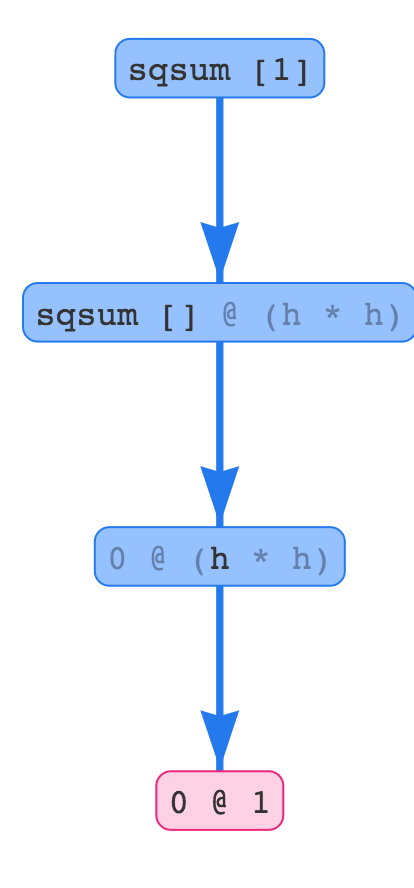
\includegraphics[height=125px]{sqsum.png}
\end{center}
%
Note how the eye is drawn to the entire stuck term as opposed to just
the left sub-term. This emphasizes the \emph{conflict} between @int@ and
@list@ rather than assuming one or the other is correct.

Next we consider a function @sumList@ that just sums the elements of the
input list, but has a more unfortunate error.
\begin{ecode}
  let rec sumList xs = match xs with
    | []    -> []
    | y::ys -> y + __sumList ys__
\end{ecode}
%
In this case the student has returned @[]@ in the base case instead of
@0@. Unfortunately, \ocaml deduces (incorrectly) from the base case that
@sumList@ must return a @list@, and then proceeds to blame the
\emph{recursive call} on line 3 for producing a @list@ instead of an
@int@.
%
\begin{verbatim}
  This expression has type
    'a list
  but an expression was expected of type
    int
\end{verbatim}
%
\toolname's jump compressed trace shows how the evaluation of
@sumList [1; 2]@ gets stuck when it tries to evaluate @2 + []@.
%
\begin{center}
  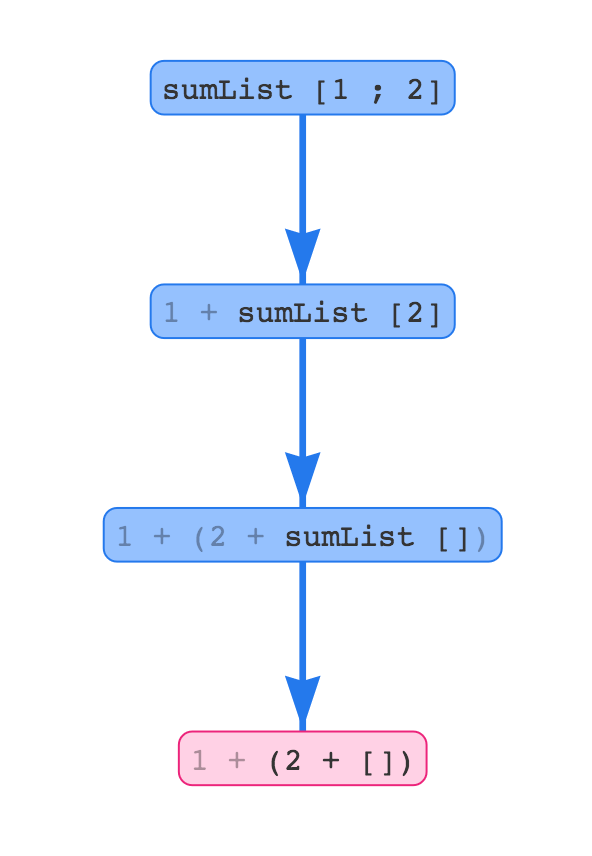
\includegraphics[height=125px]{sumlist.png}
\end{center}
%
This is essentially the same error that \ocaml produces, but the trace
clarifies immediately (via the third step) that the @[]@ is the result
of the recursive call @sumList []@, drawing attention to the incorrect
base case.

%% ES: append is actually a bit problematic as we don't find the nice
%% append [1] [2] witness. instead we could find something like
%% append [_] [], but it's not as clear IMO
% Our next example is the @append@ function, which should concatenate the
% two input lists.
% %
% \begin{ecode}
% let append xs ys = match xs with
%   | []   -> ys
%   | h::t -> h :: __t__ :: ys
% \end{ecode}
% %
% The student has forgotten to make a recursive call to @append@, and
% instead tries to cons the tail @t@ directly onto the second list @ys@.
% Consing @h@ back onto the result causes \ocaml to attempt to construct
% the infinite type @'a = 'a list@, triggering an \emph{occurs-check}
% error.
% %
% \begin{verbatim}
% Error: This expression has type
%          'a list
%        but an expression was expected of type
%          'a
%        The type variable 'a occurs inside 'a list
% \end{verbatim}
% %
% %
% \begin{center}
%   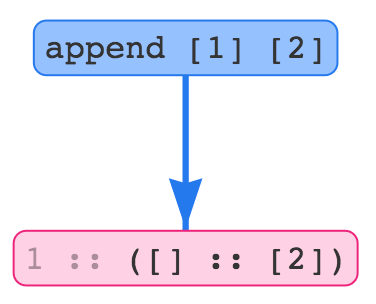
\includegraphics[height=75px]{append.png}
% \end{center}

Finally, consider the higher-order function @wwhile@ that emulates a
traditional while-loop. Concretely, @wwhile@ takes a function @f@ and
repeatedly calls @f@ on the first element of its output pair, starting
with the initial value @b@, until the second element is @false@.
%
\begin{ecode}
  let rec wwhile (f,b) =
    match f with
    | (z, false) -> z
    | (z, true)  -> wwhile (f, z)

  let f x =
    let xx = x * x in
    (xx, (xx < 100))

  let _ = wwhile (__f__, 2)
\end{ecode}
%
Unfortunately, the student has forgotten to apply @f@ at all on line 2,
and just matches it directly against a pair. This faulty definition of
@wwhile@ still typechecks however, and \ocaml thus blames the
\emph{call-site} on line 10.
%
\begin{verbatim}
  This expression has type
    int -> int * bool
  but an expression was expected of type
    'a * bool
\end{verbatim}
%
\toolname makes no assumptions about the program and quickly draws the
eye to the true error, the @match@ expression on line 2, and highlights
the conflict in matching a function against a pair pattern.
%
\begin{center}
  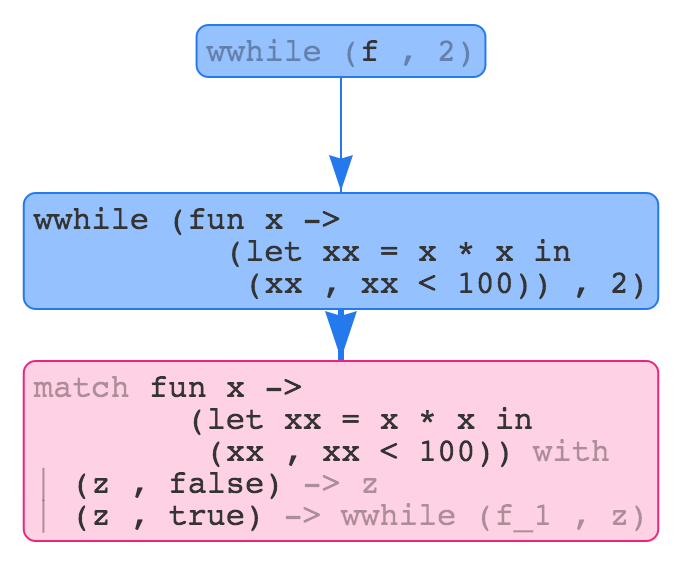
\includegraphics[height=150px]{wwhile.png}
\end{center}
%

By highlighting conflicting values rather than blaming a single value
and not making any assumptions about the given program, \toolname avoids
misleading the user into focusing their attention on a piece of code
that is actually irrelevant to the error.











%%% Local Variables:
%%% mode: latex
%%% TeX-master: "main"
%%% End:
